\documentclass{standalone}
\usepackage{tikz}
\usetikzlibrary{patterns, positioning}
\usetikzlibrary{shapes.misc}
\usepackage[outline]{contour}
\contourlength{1.5pt} 
\usepackage[sfdefault]{ClearSans} %% option 'sfdefault' activates Clear Sans as the default text font
\usepackage[T1]{fontenc}

\begin{document}
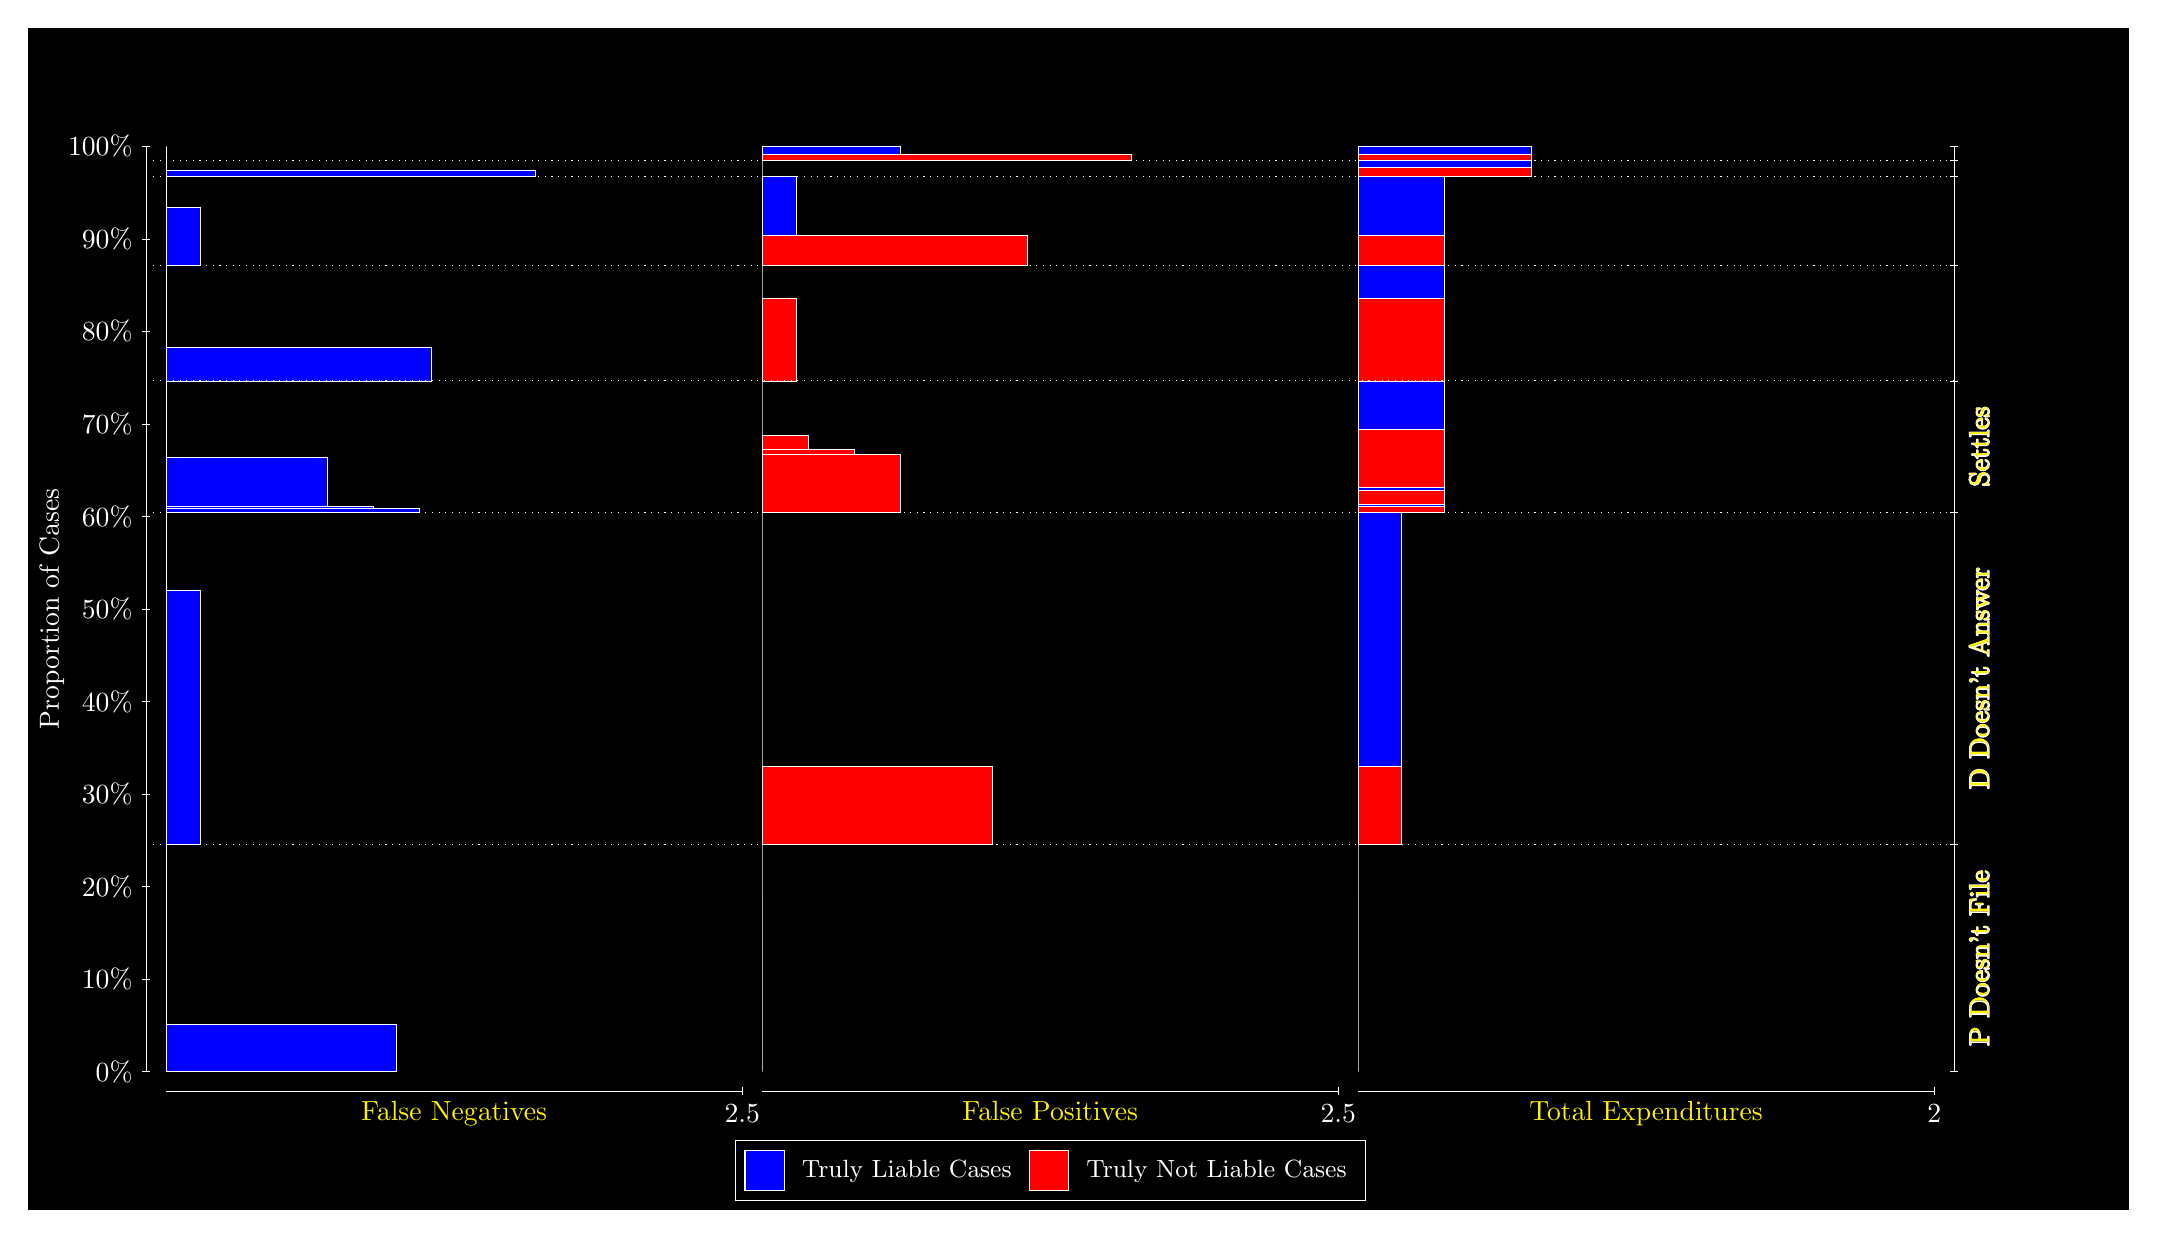
\begin{tikzpicture}
\draw[fill=black] (0,0) rectangle (26.667,15);
\draw[white, very thin] (1.5,1.75) -- (1.5,13.5);
\node[rotate=90, text=white, anchor=center] at (0.3, 7.625) {Proportion of Cases};
\draw[white, very thin] (1.45,1.75) -- (1.55,1.75);
\node[text=white, anchor=east] at (1.45, 1.75) {0\%};
\draw[white, very thin] (1.45,2.925) -- (1.55,2.925);
\node[text=white, anchor=east] at (1.45, 2.925) {10\%};
\draw[white, very thin] (1.45,4.1) -- (1.55,4.1);
\node[text=white, anchor=east] at (1.45, 4.1) {20\%};
\draw[white, very thin] (1.45,5.275) -- (1.55,5.275);
\node[text=white, anchor=east] at (1.45, 5.275) {30\%};
\draw[white, very thin] (1.45,6.45) -- (1.55,6.45);
\node[text=white, anchor=east] at (1.45, 6.45) {40\%};
\draw[white, very thin] (1.45,7.625) -- (1.55,7.625);
\node[text=white, anchor=east] at (1.45, 7.625) {50\%};
\draw[white, very thin] (1.45,8.8) -- (1.55,8.8);
\node[text=white, anchor=east] at (1.45, 8.8) {60\%};
\draw[white, very thin] (1.45,9.975) -- (1.55,9.975);
\node[text=white, anchor=east] at (1.45, 9.975) {70\%};
\draw[white, very thin] (1.45,11.15) -- (1.55,11.15);
\node[text=white, anchor=east] at (1.45, 11.15) {80\%};
\draw[white, very thin] (1.45,12.325) -- (1.55,12.325);
\node[text=white, anchor=east] at (1.45, 12.325) {90\%};
\draw[white, very thin] (1.45,13.5) -- (1.55,13.5);
\node[text=white, anchor=east] at (1.45, 13.5) {100\%};

\draw[white, very thin] (24.457,1.75) -- (24.457,13.5);
\draw[white, very thin] (24.407,1.75) -- (24.507,1.75);
\node[anchor=west] at (24.407, 1.75) {};
\draw[white, very thin] (24.407,4.633) -- (24.507,4.633);
\node[anchor=west] at (24.407, 4.633) {};
\draw[white, very thin] (24.407,8.8552) -- (24.507,8.8552);
\node[anchor=west] at (24.407, 8.8552) {};
\draw[white, very thin] (24.407,10.521) -- (24.507,10.521);
\node[anchor=west] at (24.407, 10.521) {};
\draw[white, very thin] (24.407,11.988) -- (24.507,11.988);
\node[anchor=west] at (24.407, 11.988) {};
\draw[white, very thin] (24.407,13.12) -- (24.507,13.12);
\node[anchor=west] at (24.407, 13.12) {};
\draw[white, very thin] (24.407,13.318) -- (24.507,13.318);
\node[anchor=west] at (24.407, 13.318) {};
\draw[white, very thin] (24.407,13.5) -- (24.507,13.5);
\node[anchor=west] at (24.407, 13.5) {};

\draw[white, very thin, fill=blue] (1.75,1.75) rectangle (4.6775,2.3439);
\draw[white, very thin, fill=red] (1.75,2.3439) rectangle (1.75,4.633);
\draw[white, very thin, fill=blue] (1.75,4.633) rectangle (2.1891,7.8672);
\draw[white, very thin, fill=red] (1.75,7.8672) rectangle (1.75,8.8552);
\draw[white, very thin, fill=blue] (1.75,8.8552) rectangle (4.9703,8.8979);
\draw[white, very thin, fill=blue] (1.75,8.8979) rectangle (4.3848,8.9319);
\draw[white, very thin, fill=blue] (1.75,8.9319) rectangle (3.7993,9.5491);
\draw[white, very thin, fill=red] (1.75,9.5491) rectangle (1.75,10.521);
\draw[white, very thin, fill=blue] (1.75,10.521) rectangle (5.1167,10.944);
\draw[white, very thin, fill=red] (1.75,10.944) rectangle (1.75,11.988);
\draw[white, very thin, fill=blue] (1.75,11.988) rectangle (2.1891,12.732);
\draw[white, very thin, fill=red] (1.75,12.732) rectangle (1.75,13.12);
\draw[white, very thin, fill=blue] (1.75,13.12) rectangle (6.4341,13.199);
\draw[white, very thin, fill=red] (1.75,13.199) rectangle (1.75,13.318);
\draw[white, very thin, fill=red] (1.75,13.318) rectangle (1.75,13.394);
\draw[white, very thin, fill=blue] (1.75,13.394) rectangle (1.75,13.5);
\draw[white, very thin, fill=red] (9.3189,1.75) rectangle (9.3189,4.0391);
\draw[white, very thin, fill=blue] (9.3189,4.0391) rectangle (9.3189,4.633);
\draw[white, very thin, fill=red] (9.3189,4.633) rectangle (12.246,5.621);
\draw[white, very thin, fill=blue] (9.3189,5.621) rectangle (9.3189,8.8552);
\draw[white, very thin, fill=red] (9.3189,8.8552) rectangle (11.075,9.5868);
\draw[white, very thin, fill=red] (9.3189,9.5868) rectangle (10.49,9.6549);
\draw[white, very thin, fill=red] (9.3189,9.6549) rectangle (9.9044,9.8266);
\draw[white, very thin, fill=blue] (9.3189,9.8266) rectangle (9.3189,10.521);
\draw[white, very thin, fill=red] (9.3189,10.521) rectangle (9.758,11.564);
\draw[white, very thin, fill=blue] (9.3189,11.564) rectangle (9.3189,11.988);
\draw[white, very thin, fill=red] (9.3189,11.988) rectangle (12.686,12.375);
\draw[white, very thin, fill=blue] (9.3189,12.375) rectangle (9.758,13.12);
\draw[white, very thin, fill=red] (9.3189,13.12) rectangle (9.3189,13.239);
\draw[white, very thin, fill=blue] (9.3189,13.239) rectangle (9.3189,13.318);
\draw[white, very thin, fill=red] (9.3189,13.318) rectangle (14.003,13.394);
\draw[white, very thin, fill=blue] (9.3189,13.394) rectangle (11.075,13.5);
\draw[white, very thin, fill=red] (16.888,1.75) rectangle (16.888,4.0391);
\draw[white, very thin, fill=blue] (16.888,4.0391) rectangle (16.888,4.633);
\draw[white, very thin, fill=red] (16.888,4.633) rectangle (17.437,5.621);
\draw[white, very thin, fill=blue] (16.888,5.621) rectangle (17.437,8.8552);
\draw[white, very thin, fill=red] (16.888,8.8552) rectangle (17.986,8.9233);
\draw[white, very thin, fill=blue] (16.888,8.9233) rectangle (17.986,8.9572);
\draw[white, very thin, fill=red] (16.888,8.9572) rectangle (17.986,9.129);
\draw[white, very thin, fill=blue] (16.888,9.129) rectangle (17.986,9.1717);
\draw[white, very thin, fill=red] (16.888,9.1717) rectangle (17.986,9.9033);
\draw[white, very thin, fill=blue] (16.888,9.9033) rectangle (17.986,10.521);
\draw[white, very thin, fill=red] (16.888,10.521) rectangle (17.986,11.564);
\draw[white, very thin, fill=blue] (16.888,11.564) rectangle (17.986,11.988);
\draw[white, very thin, fill=red] (16.888,11.988) rectangle (17.986,12.375);
\draw[white, very thin, fill=blue] (16.888,12.375) rectangle (17.986,13.12);
\draw[white, very thin, fill=red] (16.888,13.12) rectangle (19.083,13.239);
\draw[white, very thin, fill=blue] (16.888,13.239) rectangle (19.083,13.318);
\draw[white, very thin, fill=red] (16.888,13.318) rectangle (19.083,13.394);
\draw[white, very thin, fill=blue] (16.888,13.394) rectangle (19.083,13.5);
\draw[white, dotted] (1.5,4.633) -- (24.457,4.633);
\draw[white, dotted] (1.5,8.8552) -- (24.457,8.8552);
\draw[white, dotted] (1.5,10.521) -- (24.457,10.521);
\draw[white, dotted] (1.5,11.988) -- (24.457,11.988);
\draw[white, dotted] (1.5,13.12) -- (24.457,13.12);
\draw[white, dotted] (1.5,13.318) -- (24.457,13.318);
\draw[white, very thin] (1.75,1.5) -- (9.0689,1.5);
\node[text=yellow, anchor=north] at (5.4094, 1.5) {False Negatives};
\draw[white, very thin] (9.0689,1.45) -- (9.0689,1.55);
\node[text=white, anchor=north] at (9.0689, 1.45) {2.5};

\draw[white, very thin] (9.3189,1.5) -- (16.638,1.5);
\node[text=yellow, anchor=north] at (12.978, 1.5) {False Positives};
\draw[white, very thin] (16.638,1.45) -- (16.638,1.55);
\node[text=white, anchor=north] at (16.638, 1.45) {2.5};

\draw[white, very thin] (16.888,1.5) -- (24.207,1.5);
\node[text=yellow, anchor=north] at (20.547, 1.5) {Total Expenditures};
\draw[white, very thin] (24.207,1.45) -- (24.207,1.55);
\node[text=white, anchor=north] at (24.207, 1.45) {2};

\node[text=yellow, centered, rotate=90] at (24.777, 3.1915) {\contour{white}{P Doesn't File}};
\node[text=yellow, centered, rotate=90] at (24.777, 6.7441) {\contour{white}{D Doesn't Answer}};
\node[text=yellow, centered, rotate=90] at (24.777, 9.6878) {\contour{white}{Settles}};





\draw (12.978300999999998,1.5) node[draw=none] (baseCoordinate) {};
\begin{scope}[align=center]
        \matrix[scale=0.5, draw=white, below=0.5cm of baseCoordinate, nodes={draw}, column sep=0.1cm]{
            \node[rectangle, draw, minimum width=0.5cm, minimum height=0.5cm, fill=blue] {}; &
            \node[draw=none, font=\small, text=white] (B) {Truly Liable Cases}; &
            \node[rectangle, draw, minimum width=0.5cm, minimum height=0.5cm, fill=red] {}; &
            \node[draw=none, font=\small, text=white] (B) {Truly Not Liable Cases}; \\
            };
\end{scope}

\end{tikzpicture}
\end{document}